\pdfminorversion=7
%%
%% This is file `sample-sigconf.tex',
%% generated with the docstrip utility.
%%
%% The original source files were:
%%
%% samples.dtx  (with options: `sigconf')
%% 
%% IMPORTANT NOTICE:
%% 
%% For the copyright see the source file.
%% 
%% Any modified versions of this file must be renamed
%% with new filenames distinct from sample-sigconf.tex.
%% 
%% For distribution of the original source see the terms
%% for copying and modification in the file samples.dtx.
%% 
%% This generated file may be distributed as long as the
%% original source files, as listed above, are part of the
%% same distribution. (The sources need not necessarily be
%% in the same archive or directory.)
%%
%% The first command in your LaTeX source must be the \documentclass command.
\documentclass[sigconf]{acmart}
\usepackage[british]{babel}
%\usepackage[noadjust]{cite}
\usepackage{url}
\usepackage[hyphenbreaks]{breakurl}
\usepackage{booktabs}
\usepackage{multirow}
\usepackage{lscape}
\usepackage{acmart-taps}
\usepackage{graphicx}
\def\UrlBreaks{\do\/\do-}
%\newcommand\notype[1]{\unskip}

%\usepackage{balance}

%%
%% \BibTeX command to typeset BibTeX logo in the docs
\AtBeginDocument{%
  \providecommand\BibTeX{{%
    \normalfont B\kern-0.5em{\scshape i\kern-0.25em b}\kern-0.8em\TeX}}}

%% Rights management information.  This information is sent to you
%% when you complete the rights form.  These commands have SAMPLE
%% values in them; it is your responsibility as an author to replace
%% the commands and values with those provided to you when you
%% complete the rights form.

%% These commands are for a PROCEEDINGS abstract or paper.
\copyrightyear{2020} 
\acmYear{2020} 
\setcopyright{acmcopyright}\acmConference[UKICER '20]{United Kingdom \& Ireland Computing Education Research conference.}{September 3--4, 2020}{Glasgow, United Kingdom}
\acmBooktitle{United Kingdom \& Ireland Computing Education Research conference. (UKICER '20), September 3--4, 2020, Glasgow, United Kingdom}
\acmPrice{15.00}
\acmDOI{10.1145/3416465.3416472}
\acmISBN{978-1-4503-8849-8/20/09}


%%
%% Submission ID.
%% Use this when submitting an article to a sponsored event. You'll
%% receive a unique submission ID from the organizers
%% of the event, and this ID should be used as the parameter to this command.
%%\acmSubmissionID{123-A56-BU3}

%%
%% The majority of ACM publications use numbered citations and
%% references.  The command \citestyle{authoryear} switches to the
%% "author year" style.
%%
%% If you are preparing content for an event
%% sponsored by ACM SIGGRAPH, you must use the "author year" style of
%% citations and references.
%% Uncommenting
%% the next command will enable that style.
%%\citestyle{acmauthoryear}

%%
%% end of the preamble, start of the body of the document source.
\begin{document}

%%
%% The "title" command has an optional parameter,
%% allowing the author to define a "short title" to be used in page headers.
\title[Impact of COVID-19 on the UK Computer Science Education Community]{The Impact of COVID-19 and ``Emergency Remote Teaching'' on the UK Computer Science Education Community}

%%
%% The "author" command and its associated commands are used to define
%% the authors and their affiliations.
%% Of note is the shared affiliation of the first two authors, and the
%% "authornote" and "authornotemark" commands
%% used to denote shared contribution to the research.

\author{Tom Crick}
\orcid{0000-0001-5196-9389}
\affiliation{%
  \institution{Swansea University}
  \city{Swansea}
  \country{UK}
}
\email{thomas.crick@swansea.ac.uk}

\author{Cathryn Knight}
\orcid{0000-0002-7574-3090}
\affiliation{%
  \institution{Swansea University}
  \city{Swansea}
  \country{UK}
}
  \email{cathryn.knight@swansea.ac.uk}

\author{Richard Watermeyer}
\orcid{0000-0002-2365-3771}
\affiliation{%
  \institution{University of Bristol}
  \city{Bristol}
  \country{UK}
}
\email{richard.watermeyer@bristol.ac.uk}

\author{Janet Goodall}
\orcid{0000-0002-0172-2035}
\affiliation{%
  \institution{Swansea University}
  \city{Swansea}
  \country{UK}
}
  \email{j.s.goodall@swansea.ac.uk}

%% By default, the full list of authors will be used in the page
%% headers. Often, this list is too long, and will overlap
%% other information printed in the page headers. This command allows
%% the author to define a more concise list
%% of authors' names for this purpose.
\renewcommand{\shortauthors}{Crick, et al.}

%%
%% The abstract is a short summary of the work to be presented in the
%% article.
\begin{abstract}
The COVID-19 pandemic has imposed ``emergency remote teaching'' across
education globally, leading to the closure of institutions across a
variety of settings, from early-years through to higher
education. This paper looks specifically at the impact of these
changes to those teaching the discipline of computer science in the
UK. Drawing on the quantitative and qualitative findings from a
large-scale survey of the educational workforce (N=2,197) conducted in
the immediate aftermath of institutional closures in March 2020 and
the shift to online delivery, we report how those teaching computer
science in various UK settings (n=214) show significantly more
positive attitudes towards the move to online learning, teaching and
assessment than those working in other disciplines; these perceptions
were consistent across schools, colleges and higher education
institutions. However, whilst practitioners noted the opportunities of
these changes for their respective sector -- especially a renewed
focus on the importance of digital skills -- they raised a number of
generalisable concerns on the impact of this shift to online on their
roles, their institutions and their sectors as a whole; for example,
the impact on workload, effective pedagogy and job fragility. More
specifically for computer science practitioners, curricula and
qualifications, there were concerns raised regarding the ability to
meaningfully deliver certain core topics such as mathematical
foundations and programming, as well as the impact on various types of
formal examinations and assessment. Based on the data obtained from
this rapid response survey, we offer informed commentary, evaluation
and recommendations for emerging learning and teaching policy and
practice in the UK computer science community as we move into the
2020-2021 academic year and beyond.
\end{abstract}

%%
%% The code below is generated by the tool at http://dl.acm.org/ccs.cfm.
%% Please copy and paste the code instead of the example below.
%%
\begin{CCSXML}
<ccs2012>
<concept>
<concept_id>10003456.10003457.10003527</concept_id>
<concept_desc>Social and professional topics~Computing education</concept_desc>
<concept_significance>500</concept_significance>
</concept>
<concept>
<concept_id>10003456.10010927</concept_id>
<concept_desc>Social and professional topics~User characteristics</concept_desc>
<concept_significance>500</concept_significance>
</concept>
<concept>
<concept_id>10002944.10011123.10010912</concept_id>
<concept_desc>General and reference~Empirical studies</concept_desc>
<concept_significance>500</concept_significance>
</concept>
</ccs2012>
\end{CCSXML}

\ccsdesc[500]{Social and professional topics~Computing education}
\ccsdesc[500]{Social and professional topics~User characteristics}
\ccsdesc[500]{General and reference~Empirical studies}

%%
%% Keywords. The author(s) should pick words that accurately describe
%% the work being presented. Separate the keywords with commas.
\keywords{COVID-19, emergency remote teaching, practitioner
perceptions, pedagogy, assessment, curriculum, computer science
education}

%%
%% This command processes the author and affiliation and title
%% information and builds the first part of the formatted document.
\maketitle

\section{Introduction}\label{intro}

\subsection{The Impact of COVID-19}

The impact of the COVID-19 (SARS-CoV-2) global pandemic is currently
incalculable; it has affected, and continues to affect, profound
social suffering, significant cultural disruption, and deep economic
hardship. While indiscriminate in terms of whom it infects, it has
largely punished society’s most vulnerable and less
fortunate~\cite{vonbraun-et-al:2020,lancetcovid:2020,vanlancker+parolin:2020};
worse now, it appears that the virus may have to be tolerated on an
indefinite basis~\cite{kissler-et-al:2020}.

The impact of the pandemic on the wider education system, across all
settings, has been
profound~\cite{unescocovidedu:2020,armitage+nellums:2020}, presenting
significant challenges for learning, teaching and assessment (LT\&A),
especially from a pedagogic
perspective~\cite{doucet-et-al:2020,oecd:2020,aace:2020} -- and how
face-to-face learning is somehow perceived to be ``better value'' than
online approaches~\cite{paechter+maier:ihe2010,scbbcnews:2020}. In the
United Kingdom (UK), there have been major responses from governments,
organisations and institutions at all levels and settings; from major
national policy initiatives to support learners and maintain quality
and standards across all settings, to ongoing government inquiries on
the longer-term impact of COVID-19 on education and children’s
services.

% \footnote{e.g. in Wales \url{https://business.senedd.wales/mgConsultationDisplay.aspx?ID=392}}
% ~\cite{hocedu:2020,seneddcype:2020}.
% ~\cite{qaaqands:2020}
% ~\footnote{e.g. in Wales ``{\emph{Stay Safe. Stay Learning: supporting the education
% system}}''
% \url{https://gov.wales/stay-safe-stay-learning-supporting-education-system-html}},
% in England: ``{\emph{Guidance for schools: coronavirus (COVID-19)}}''
% \url{https://www.gov.uk/government/collections/guidance-for-schools-coronavirus-covid-19}

\subsection{Educational Technology and Digital Learning}

The general impact and efficacy of educational technology and digital
learning is still uncertain in the formal academic literature, being
dependent on specific educational settings and LT\&A context. Whilst a
range of international research studies have shown benefits of the
successful application of digital LT\&A across a variety of contexts
and settings, the widespread adoption, implementation and evaluation
of educational technologies has yet to be fully
realised~\cite{decodinglearning:2012,means:2014,ecjrc:2017,mayer:2018}.
The research and policy debate regarding the efficacy, utility and
impact of educational technology and digital practice is ongoing,
reinforced by a national digital learning and teaching strategy in
Scotland~\cite{digscot:2016}, a new Digital Competence Framework for
all learners aged 3-16 in
Wales~\cite{wgictreview:2013,wgdcfguidance:2018}, a new national
strategy for schools in England~\cite{dfe:2019}, as well as recent
work from Jisc (a not-for-profit organisation that provides digital
solutions for UK education and research) on digital practice in
further education (FE) and higher education
(HE)~\cite{jisc:2020}, and from the UK's Quality Assurance
Agency on a taxonomy for digital
learning~\cite{qaadigtaxonomy:2020}. We have also seen updated
guidance on how digital learning can support learning, as well as a
rapid evidence assessment on remote learning from the Education
Endowment Foundation~\cite{eefdigtech:2019,eefremote:2020}.\vspace*{-2pt}

\subsection{The Discipline of Computer Science}

% examples: http://www.cs.ox.ac.uk/innovation/covid-19/
% ~\cite{bcs:2020}
It is clear that the academic discipline of computer science -- and
indeed the wider information technology sector -- has
much to offer to address the wider challenges resulting from the
COVID-19 pandemic; from computational modelling, the use of AI,
machine learning and big data, as well as the wider legal, social,
ethical and professional issues, such as from contact tracing,
personal data sharing/storage, and the use of image recognition and
surveillance~\cite{dwivedi-et-al:ijim2019,ting-et-al:2020,cerf:2020,chun-et-al:2020,rcjbbcnews:2020}. There
has also been recent analysis on the impact of COVID-19 on the
computer science research community -- as we have seen across
international scientific research communities more
broadly~\cite{oecdcovid19:2020} -- especially on ongoing projects,
careers, and dissemination of work~\cite{msrcovid19:2020}. However,
there has been little focus on what this means for computer science
education and practitioners, especially thinking about the range of
specific disciplinary challenges for LT\&A, across all settings and
levels. This directly links to recent significant changes to computer
science curricula, qualifications and practice across the
UK~\cite{brown-et-al-toce2014,davenport-et-al:latice2016,
murphy-et-al:programming2017, rscsedproject:2017}, as well as
the emerging focus on the required digital skills and infrastructure
to support the UK's post-COVID economic
renewal~\cite{tryfonas+crick:petra2018,crick-et-al:fie2019,davenport-et-al:educon2020}.\vspace*{-2pt}
% Also linking back to recent work on CS/STEM curriculum reform, digital
% skills, accreditation, etc
% CS specific context: shifts in the discipline, school curriculum
% reform, wider digital economy, high-value digital skills across the UK
% https://teachcomputing.org/

% Data collected in the Immediate aftermath of the lockdown and
% shift to online, recognising this is a limitation, but this links to
% planning and preparation for next academic, supporting emerging policy
% and practice. i.e. what we can learn from this, how might the
% sector/discipline change as a result?
% Impact on practitioners, institutions and their respective
% sectors, with derived/implied impact on students.

% Research question: “How do computer scientists in the field of
% education perceive the rapid shift to ERT?”
\subsection{Motivation}

We thus undertook a survey of UK computer scientists on their
perspectives as practitioners on the rapid shift to ``emergency remote
teaching'' and transitioning online at the height of the COVID-19
crisis, and what they identify and forecast as its immediate and
prospective impacts. The data was collected in the immediate aftermath
of the forced institutional lockdowns and shift to online LT\&A. It
aimed to provide insight into emerging policy and practice; impact on
practitioners, institutions and thus students; how might this change
the discipline as a result; and what might this mean for the coming
academic year and the longer-term.  The discussion that follows is
based upon the perspectives of n=214 practitioners (as part of a
larger survey of the educational workforce (N=2,197), including
specific work on the UK higher education
sector in the UK~\cite{watermeyer-et-al:he2020}) drawn from across all
educational settings, institutions, and the career hierarchy, and what
they recognise to be the major consequences of COVID-19, the
transition to online LT\&A, and the challenges of maintaining
``continuity of learning''. Their accounts document the hopes and
fears of the UK computer science education community in the face of
seismic and, as may prove to be, inalterable shifts. The majority of
respondents tend towards a significantly more positive view of online
migration than those working in other disciplines, recognising the
opportunities and potential affordances of the crisis; these
perceptions were consistent across all educational settings. There
were some, albeit a minority, who raised a number of generalisable
concerns on the impact of this shift to online and the challenges
relating to their roles, their institutions and their sectors as a
whole.

\subsubsection*{A Note on Terminology}

While in many instances throughout this paper we will refer to the UK
-- consisting of the four nations of England, Scotland, Wales and
Northern Ireland -- we will attempt to be as clear as possible when
referring to specific policies or initiatives across or between the
nations, as a number of policy areas, including education and skills,
are devolved to the respective national governments. However, for the
purposes of this study, we will be looking at aggregated UK-level
impacts and perceptions of computer science practitioners.

With regards to the consistent naming of the discipline through this
paper, we use ``computer science'' to refer to the wider cognate
discipline as represented by ICT, computing and informatics across
schools, FE and HE in the UK.\vspace*{-2pt}

\section{Methods}\label{methods}

\subsection{Sample}

The survey aimed to investigate how the UK computer science education
workforce has viewed the move to online LT\&A. The target population was
those who are actively involved in the delivery of LT\&A within the
education sector. Those who did not meet this criterion were excluded
from analysis post-hoc.

We adopted a convenience sampling approach in distributing the
Qualtrics survey whereby a link to the survey was shared via mailing
lists of professional networks and related education organisations
(for example, via the Council for Professors and Heads of Computing
(CPHC), BCS Academy, ACM SIGCSE, the UK's University and College Union
(UCU), and the British Educational Research Association (BERA) Higher
Education Special Interest Group, in addition to Twitter and
LinkedIn). While the use of convenience sampling does not allow
generalisation to a representative population, this sampling technique
allowed us to document patterns within the observed population, with
minimal time and cost restrictions.

After excluding those that did not meet the participant requirements
2,197 members of the UK education workforce responded to the
survey. This included 1,148 respondents from the HE (university)
sector (52.3\%), 279 respondents from FE (12.7\%) and 569 respondents
from schools (25.9\%). 214 participants indicated that they taught
computer science. This included 119 from the HE sector (55.6\%), 24
from FE (11.2\%) and 71 from schools (33.2\%).

The survey was launched on 26 March 2020 following the announcement of
closures across all educational settings in all four nations of the
UK, and remained open for four weeks. Due to the distribution method
we cannot calculate the response rate; however, of those who started
the survey, 84.9\% completed it.

\subsection{Questionnaire}

On the first page of the questionnaire respondents were informed that
the research was designed to identify their views and experiences of
the move to online LT\&A in response to COVID-19. The first section of
the questionnaire consisted of demographic questions in order to
determine how participant characteristics impacted key variables. In
order to identify those who are computer scientists, those who
responded that they worked in the HE sector were asked to select their
discipline from a list created using the UK Joint Academic Coding of
Subjects (JACS)
codes\footnote{\url{https://www.hesa.ac.uk/support/documentation/jacs}}. Those
who worked in schools and FE were firstly asked if they taught a
particular subject. Those that responded that they did were then asked
to select their subject from a list containing all curriculum subjects
taught across the four nations of the UK.

Demographic questions were followed by Likert and slider-scale
questions exploring respondents' views of the changes. These included
questions about how prepared and confident they felt about the move to
online teaching. In addition, respondents were asked three open-ended questions in
order to gain their overall insight into the impact of the changes:
``{\emph{Please provide any comments of how the online learning and
teaching changes brought in as a response to COVID-19 will impact
upon}}'' followed by ``{\emph{your role}}'', ``{\emph{your
institution}}'' and ``{\emph{your sector of education}}''.

Ethical approval for this study was obtained from Swansea University's
College of Arts and Humanities Research Ethics Committee. The survey
was piloted on a subsample of the population before distribution to
the wider UK computer science workforce.

\subsection{Analysis}

Quantitative bivariate chi-square (($\chi^2$)) analysis of the key
variables was conducted in order to determine overall attitudes to
online LT\&A and whether there were significant differences between
those in computer science and those in other disciplines. Chi-square
tests were utilised due to the categorical nature of the variables and
to assess whether the observed cell counts are significantly different
from the expected cell counts. As there were more participants from
computer science that responded from HE institutions it was necessary
to control for the effect of setting on these outcomes. Furthermore,
it could be hypothesised that variables such as gender and years
working in education may have also predict the participants responses
to these questions. Therefore, binary logistic regression was used in
order to control for these variables.

Qualitative analysis of the open-ended questions used thematic
analysis. Thematic analysis has been described as ``a method for
identifying, analysing and reporting patterns (themes) within
data''~\cite[p.78]{braun+clarke:2006}. This was done by firstly
reading through the qualitative responses and numerically coding the
data to identify whether comments were positive, negative or
neutral. The responses were coded by two researchers to ensure
inter-rater reliability (IRR=0.82). Within these codes potential
themes were identified: ``a theme captures something important about
the data in relation to the research question and represents some
level of patterned response or meaning within the data
set''~\cite[p.82]{braun+clarke:2006}. These themes were reviewed
rigorously against the data to ensure that they were compatible with
the data and accurately represented the comments.

\section{Results}\label{results}

\subsection{Quantitative Data}\label{quantdata}

Figure~\ref{fig:partagree} shows that those who work within the
computer science discipline were significantly more likely to say
that they felt prepared ($\chi^2$(1)= 22.02, p<0,001), confident
($\chi^2$(1)= 22.98, p<0,001), supported by their institution
($\chi^2$(1)= 4.5, p=0.03), held a good working knowledge of
appropriate technologies ($\chi^2$(1)= 47.75, p<0,001), had access to
appropriate technologies ($\chi^2$(1)= 13.19, p<0,001) and were
confident that their students could access online LT\&A ($\chi^2$(1)=
17.16, p<0,001).

\begin{figure*}
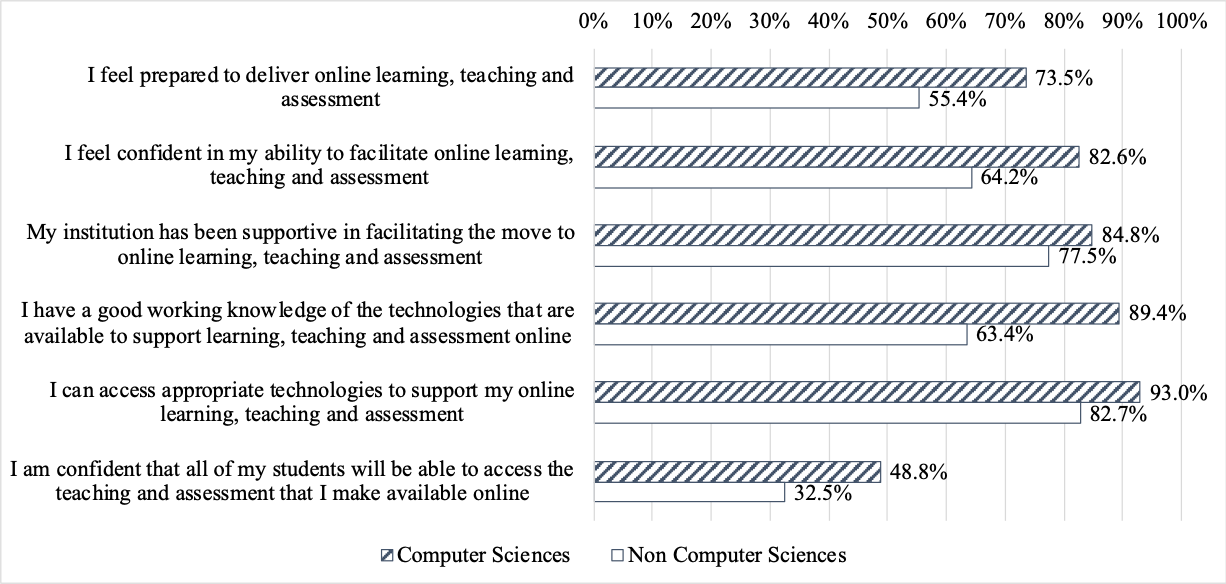
\includegraphics[width=0.8\textwidth]{particagree.png}
\caption{Percentage of participants that agree to statements about
  online LT\&A}
\label{fig:partagree}
\end{figure*}

Table~\ref{tab:binregs} shows the results from binary regression on each
statement. This demonstrates that the impact of working within the
computer science discipline remains significant when controlling for
setting, gender, and years teaching. It also shows that those in
schools were significantly more likely to agree with the statements
than those in HE and FE.

%\begin{landscape}
\begin{table*}[]
\caption{Binary regressions on key survey statements}
\begin{imageonly}
\resizebox{\textwidth}{!}{%
\begin{tabular}{@{}llllllllllllllllllllllllll@{}}
\toprule
  Variable & Category & \multicolumn{4}{l}{\textit{\begin{tabular}[c]{@{}l@{}}``I feel prepared to deliver\\ online LT\&A''\end{tabular}}} & \multicolumn{4}{l}{\textit{\begin{tabular}[c]{@{}l@{}}``I feel confident in my ability\\ to facilitate online LT\&A''\end{tabular}}} & \multicolumn{4}{l}{\textit{\begin{tabular}[c]{@{}l@{}}``My institution has been\\ supportive in facilitating\\ the move to online LT\&A''\end{tabular}}} & \multicolumn{4}{l}{\textit{\begin{tabular}[c]{@{}l@{}}``I have a good working\\ knowledge of the technologies\\ that are available to support\\ online LT\&A''\end{tabular}}} & \multicolumn{4}{l}{\textit{\begin{tabular}[c]{@{}l@{}}``I can access appropriate\\technologies to support my\\ online LT\&A''\end{tabular}}} & \multicolumn{4}{l}{\textit{\begin{tabular}[c]{@{}l@{}}``I am confident that all of my\\ students will be able to access\\ the teaching and assessment\\that I make available online''\end{tabular}}} \\ \midrule

  &  & $\beta$ & SE & p & \begin{tabular}[c]{@{}l@{}}Odds\\ Ratio\end{tabular} & $\beta$ & SE & p & \begin{tabular}[c]{@{}l@{}}Odds\\ Ratio\end{tabular} & $\beta$ & SE & p & \begin{tabular}[c]{@{}l@{}}Odds\\ Ratio\end{tabular} & $\beta$ & SE & p & \begin{tabular}[c]{@{}l@{}}Odds\\ Ratio\end{tabular} & $\beta$ & SE & p & \begin{tabular}[c]{@{}l@{}}Odds\\ Ratio\end{tabular} & $\beta$ & SE & p & \begin{tabular}[c]{@{}l@{}}Odds\\ Ratio\end{tabular} \\ \addlinespace

 \multirow{2}{*}{CS} & Non CS (ref) &  &  &  &  &  &  &  &  &  &  &  &  &  &  &  &  &  &  \\
 & CS & -0.77 & 0.19 & \textless{}0.001 & 0.46 & -0.92 & 0.22 & \textless{}0.001 & 0.4 & -0.7 & 0.14 & 0.04 & 0.61 & -1.59 & 0.27 & \textless{}0.001 & 0.20 & -0.94 & 0.32 & 0.003 & 0.39 & -0.59 & 0.18 & \textless{}0.001 & 0.55\\ \addlinespace

  \multirow{2}{*}{Gender} & Male (ref) &  &  &  &  &  &  &  &  &  &  &  &  &  &  &  &  &  &  \\
 & Female & 0.32 & 0.11 & 0.005 & 1.37 & 0.35 & 0.12 & 0.005 & 1.42 & -0.07 & 0.14 & 0.6 & 0.93 & 0.40 & 0.13 & 0.002 & 1.50 & 0.23 & 0.16 & 0.136 & 1.26 & 0.37 & 0.12 & 0.002 & 1.45 \\ \addlinespace

  \multirow{6}{*}{\begin{tabular}[c]{@{}l@{}}Years\\ working\end{tabular}} & 0-5 (ref) &  &  &  &  &  &  &  &  &  &  &  &  &  &  &  &  &  &  \\
 & 6-10 & -0.12 & 0.19 & 0.53 & 0.89 & -0.29 & 0.20 & 0.15 & 0.75 & 0.12 & 0.24 & 0.61 & 1.13 & -0.01 & 0.20 & 0.98 & 1.00 & 0.22 & 0.26 & 0.4 & 1.24 & 0.01 & 0.20 & 0.981 & 1.01\\
 & 11-15 & -0.0 & 0.18 & 0.99 & 0.99 & 0.02 & 0.2 & 0.89 & 1.03 & 0.51 & 0.22 & 0.02 & 1.66 & 0.08 & 0.20 & 0.68 & 1.08 & 0.29 & 0.25 & 0.25 & 1.33 & 0.06 & 0.19 & 0.759 & 1.06\\
 & 16-20 & 0.06 & 0.19 & 0.76 & 1.06 & 0.00 & 0.2 & 0.99 & 1.00 & 0.47 & 0.23 & 0.45 & 1.60 & 0.24 & 0.21 & 0.26 & 1.27 & 0.31 & 0.26 & 0.24 & 1.36 & 0.04 & 0.20 & 0.829 & 1.04\\
 & 21-25 & 0.25 & 0.19 & 0.18 & 1.29 & 0.20 & 0.20 & 0.31 & 1.22 & 0.32 & 0.25 & 0.19 & 1.38 & 0.47 & 0.21 & 0.02 & 1.60 & 0.73 & 0.25 & 0.01 & 2.08 & -0.03 & 0.20 & 0.865 & 0.97\\
 & 26+ & 0.39 & 0.19 & 0.04 & 1.48 & 0.36 & 0.20 & 0.08 & 1.43 & 0.31 & 0.24 & 0.19 & 1.37 & 0.65 & 0.22 & 0.003 & 1.91 & 0.20 & 0.28 & 0.50 & 1.22 & 0.00 & 0.20 & 0.997 & 1.00\\ \addlinespace

  \multirow{3}{*}{Setting} & School (ref) &  &  &  &  &  &  &  &  &  &  &  &  &  &  &  &  &  &  \\
 & FE & 0.67 & 1.78 & \textless{}0.001 & 1.96 & 0.76 & 0.19 & \textless{}0.001 & 2.14 & 0.61 & 0.24 & 0.01 & 1.84 & 0.85 & 0.20 & \textless{}0.001 & 2.35 & 0.70 & 0.24 & 0.004 & 2.01 & -0.23 & 0.19 & 0.235 & 0.80\\
 & HE & 1.08 & 0.11 & \textless{}0.001 & 2.94 & 0.94 & 0.14 & \textless{}0.001 & 2.55 & 1.07 & 0.24 & \textless{}0.001 & 2.92 & 1.14 & 0.15 & \textless{}0.01 & 3.11 & 0.78 & 0.19 & \textless{}0.001 & 2.18 & -0.56 & 0.14 & \textless{}0.001 & 0.57\\ \addlinespace

  \multicolumn{2}{l}{Constant} & -1.29 & 0.19 & \textless{}0.001 & 0.28 & -1.55 & 0.20 & \textless{}0.001 & 0.21 & -2.29 & 0.25 & \textless{}0.001 & 0.10 & -1.86 & 0.22 & \textless{}0.001 & 0.16 & -2.65 & 0.27 & \textless{}0.001 & 0.07 & 0.82 & 0.19 & \textless{}0.001 & 2.26\\ \bottomrule
\end{tabular}%
}
\end{imageonly}
\label{tab:binregs}
\vspace*{-5pt}\end{table*}
%\end{landscape}

\subsection{Qualitative Data}\label{qualdata}

The qualitative data were coded into positive, negative and neutral
responses. Of the 102 computer scientists that commented on the impact
on their role 23 (22.6\%) were positive, 54 (52.9\%) were negative and
25 (24.5\%) were neutral.  94 computer scientists provided a comment
on the impact on their institution, of these 20 (21.3\%) were
positive, 59 (56.7\%) were negative and 15 (15\%) were
neutral. Finally, 67 computer scientists commented on the impact on
their sector, of these 16 (23.9\%) were positive, 36 (53.7\%) were
negative and 15 (22.4\%) neutral. Key themes were identified within
the responses. These will now be discussed in relation to computer
sciences education.

\subsubsection{Change as progressive}

\begin{quotation}
``{\emph{Computer science education is probably a good place to be
right now.}}'' [HE]
\end{quotation}

\begin{quotation}
``{\emph{We are in a pretty unique place because of what we
teach. }}'' [school]
\end{quotation}

Computer scientists mentioned a number of progressive and beneficial
aspects to the change to online LT\&A for the discipline. Most
prominently, respondents pointed out how the changes have and would
lead to more recognition of the importance of technology. Common
responses mentioned the ``{\emph{greater staff awareness of
educational technologies}}” [school] and that ``{\emph{everyone
hopefully will now appreciate that digital literacy is important}}''
[school]. This led to many respondents also recognising how computer
science as a subject may have its profile raised by the mass move to
the use of digital technology for learning. One respondent noted
``{\emph{it may put further emphasis on computing as a subject, with
so much technology in use}}'' [school]. As a result, respondents
foresaw long-term benefits for computer science as a discipline
within education ``{\emph{ICT has gone up massively as a valued skill
-- hopefully a trend that will be reflected and its impact will be
increased in terms of curriculum timetabling}}'' [school].

\begin{quotation}
``{\emph{If used and set up well, it could be amazing.  Breaking down
barriers to edtech and embracing technology for a connected student
experience}}'' [school]
\end{quotation}

Further opportunities were noted in the advance in educational digital
infrastructure. A key theme was the acknowledgement of the
``{\emph{range, quality and resilience of key digital infrastructure
and tools}}'' [HE] and how it may ``{\emph{open new opportunities to
try new online tools}}'' [school]. Furthermore, respondents mentioned
the potential positive impact of financial investment in digital
infrastructure. This was coupled with discussion of the opportunities
for professional development in the area of online LT\&A. It was
recognised that there had been ``{\emph{more ongoing support for staff
with technology}}'' [school] and this would lead to long term
benefits:\vspace*{-2pt}

\begin{quotation}
``{\emph{It will involve a forced skills upskilling in IT skills for a
number of older members of staff. […] Once over the initial hurdle, I
feel this could be of benefit long term. But this has only happened
due to significant support made available to them to support this}}''
[school]
\end{quotation}

% COVID-19 has been a lightning rod that has catalysed a lot of much
% needed changes in my institution. [HE]

There was also discussion about the positive impact this could have on
pedagogy and practice as it has ``{\emph{opened opportunities for
    flexible learning}}” [school]. Furthermore, respondents mentioned that
``{\emph{it will allow the department to be creative and be innovative
in the way lessons are presented to students}}'' [school]; therefore,
indicating potentially innovation online LT\&A methods for computer
science education.

There was also acknowledgement that while there may be difficulties in
terms of equity of access ``{\emph{computer science will be one of the
least hit as our colleagues and students are among the most capable
when it comes to operating online}}'' [HE].

\subsubsection{Change as challenge}

\begin{quotation}
``{\emph{I am concerned that my institution thinks a move online is a
move to more innovative and modern teaching, just by virtue of it
being online.}}'' [HE]
\end{quotation}

\begin{quotation}
``{\emph{HE will move increasingly to online provision, sadly. Our
technologies do not currently allow the creation and manipulation of
shared mental representations which is necessary for effective
teaching and learning of mathematics and computer science.}}'' [HE]
\end{quotation}

While acknowledgement of opportunities was clear within the
qualitative data, respondents also raised concerns about the impact of
the move to online LT\&A. A key theme within these concerns was
whether the move to online LT\&A would be as pedagogically beneficial
to the students as face to face teaching. The quote above summarise
the concern that top-down messages from institutions imply that `good
practice is online', however, there is concern that these decisions
are not pedagogically-driven. A number of respondents raised concerns
that computer science is ``{\emph{skills-based rather than fact-based.
I long ago abandoned the traditional lecture as being inappropriate
for teaching […] .  Too often, moving teaching online means moving
back to more traditional teaching styles.}}” [HE] and that
``{\emph{teaching programming techniques and complex concepts of
computer science online is difficult}}'' [school]. Furthermore, while
respondents were aware of the negative impact of the lack of
face-to-face teaching on teaching computer science, they also
acknowledged that ``{\emph{social interaction is arguably an important
component of the student experience}}'' [HE]. Thus, suggesting wider
pedagogical issues due to the lack of face-to-face teaching.

Along with a perceived negative impact on effective pedagogy due to
the move to online LT\&A, concerns were also raised about the equity
of access to the necessary resources for learning: ``{\emph{online
learning in CS is heavily dependent on pupils' home access}}''
[school]. Furthermore, concern was raised about the lack of access to
labs and computer science specific software for LT\&A: ``{\emph{access
to specialist laboratories and equipment has been curtailed. Depending
upon a student’s specialism within computer science their experience
could be more significantly affected. For example, those studying
networking or robotics}}'' [HE].

\looseness-1 Also, while respondents acknowledged the lack of necessary physical
resource as a problem for their students, many acknowledged the lack
of their own time as a key concern: ``{\emph{the main problem is not
availability of resource and support, but the time needed to acquire
skills in using them, for which there is no space in my current
role}}'' [HE]. The impact of moving resources online on workload was a
concern raised across the discipline: ``{\emph{huge uncertainty,
possibly spending all summer converting a large course to online
without knowing whether/if students will even enrol}}'' [HE]. This
concern about the fragility of the sector was particularly prominent
in respondents from HE. This was reinforced by concerns across all
sectors for the health and wellbeing of both practitioners and
students, linking back to previous comments regarding equity and
personal circumstances: ``{\emph{It makes me want to get out of
teaching computing; the amount of time that I spend at the computer
feels tiresome at the best of times, and now that there is no
face-to-face contact with students, the computer time is very
demoralising}}'' [school] and ``{\emph{My role is shifting towards
advising and away from teaching. A major challenge will be students'
mental health, not their ability to write Java code.}}'' [HE].

\section{Discussion}\label{discussion}

\begin{quotation}
``{\emph{This is the beginning of a new era. Things will never be the
same again.}}'' [HE]
\end{quotation}

\begin{quotation}
``{\emph{Computer Science will boom.}}'' [HE]
\end{quotation}

% \begin{itemize}
% \item Computer scientists are more prepared and confident and
% supported by institution compared to all other disciplines
% \item Quant this was significant across sector/gender/etc – the impact
% of being a CS is sig predictor of preparedness when controlling for
% sector/gender/years teaching, implying CS is sig variable…
% \item However, while qual data showed some positive responses there
% were a number of concerns around impact of online LT\&A and their roles going
% forward
% \end{itemize}

\subsection{Key Themes}

The quantitative data demonstrates that in the immediate aftermath of
the rapid move to online LT\&A, those working in computer science
perceived themselves as being significantly more prepared, confident,
held a good working knowledge of the relevant technologies and felt
supported by their institution than those in other
disciplines. Furthermore, they were significantly more likely to agree
that both themselves and their students could access the online
LT\&A. While those in secondary schools were significantly more
likely to agree with these statements than those in FE and HE, being a
computer scientist remained a significant predictor of these
viewpoints when controlling for setting, gender, and years working in
the profession.  These results are, perhaps, unsurprising, given the
likely proficiency of computer scientists to use technology. However,
they highlight that this confidence with technology translates to its
use for online LT\&A.

\begin{quotation}
``{\emph{As a Computing teacher, most of my resources are already
online. However, teaching programming techniques and complex concepts
of computer science online is difficult.}}'' [school]
\end{quotation}

Central to both the positive and negative commentary was the theme of
pedagogy. While some recognised the potential that moving teaching
online could allow practitioners to be `flexible' and `creative' with
their pedagogy, practitioners expressed concern about how key
foundation topics and threshold concepts in computer science can be
taught effectively without face-to-face instruction. Therefore, while some
literature has demonstrated the use of technology to enhance teaching,
a number of practitioners were concerned about its place in computer
science education, especially for key topics in computer science, such
as programming and mathematical foundations, as well as more practical
or collaborative topics such as robotics and group software projects.
% Might not want to phrase it like this- but perhaps can add literature
% in the intro which looks at effective use of tech for teaching- and
% refer back to it here.

\begin{quotation}
``{\emph{Specifically I work in an area that involves some hands on practical
projects. These cannot be replicated online, so the student experience
will be significantly changed.}}'' [HE]
\end{quotation}

% \begin{quotation}
% ``{\emph{HE will move increasingly to online provision, sadly.  Our
% technologies do not currently allow the creation and manipulation of
% shared mental representations which is necessary for effective
% teaching and learning of mathematics and computer science.}}'' [HE]
% \end{quotation}

Yet, it could also be argued that the efficiency of online teaching
may be overplayed by institutions. This may be particularly true of
the HE sector who may be rapidly moving teaching online, without the
necessary workforce development and understanding of effective online
pedagogy. As noted in the responses, there may be longer term positive
impact of this technological upskilling of the education workforce,
however, significant concerns were raised about the impact on workload
due to these changes. There were also concerns raised about top-down,
``one size fits all'' institutional approaches, rather than evaluating
and addressing disciplinary-specific challenges and supporting
appropriate pedagogic approaches.

Another theme that was acknowledged as both a challenge and an
opportunity was the impact on educational digital
infrastructure. While practitioners acknowledged the potential
opportunities of institutional financial investment in digital
infrastructure, concern was raised about equity of access to these
recourses. While it was acknowledged that computer science students
may be the least affected by this in HE, there was concern for those
that could not access appropriate technologies at home. Specifically,
a lack of access to specialist labs or software may be an issue going
forward.
% Something here? Maybe links to curriculum reform and how curriculum
% could be delivered without access to necessary technologies- or
% something more about equity and those worst hit by COVID.

\begin{quotation}
``{\emph{I teach programming and robotics.  Programming transitions
easily to online learning but Robotics does not.  It remains to be
seen if we can continue that class.}}'' [HE]
\end{quotation}

\subsection{Limitations}

It is also necessary to note limitations of this research and to
highlight potential for future research in this area. Firstly, this
study has grouped together UK computer science practitioners from
across various educational settings. It could be argued that the
difference in experience of these practitioners is vast and,
consequently, it is difficult to recognise them as a homogenous
group. However, logistic regression analysis demonstrated that even
while controlling for setting, identifying as a computer scientist was
a significant predictor of responses to the key statements. Across all
participants, secondary school practitioners were significantly more
positive than those in HE and FE. Therefore, future research should
investigate why this trend has been identified, and whether those in
HE and FE can learn from practitioners in schools about effective
methods of online LT\&A.

Secondly, as this research was conducted in the immediate aftermath of
the move to online LT\&A it could be argued that, due to the rapid
changes in the situation since March 2020, attitudes may have changed
since this data was collected. However, this research offers insight
into the education workforce’s perceptions during these radical
changes to their practices. The results highlight the longer-term
opportunities and challenges that the move may bring
about. Furthermore, follow up research should be conducted in order to
understand whether perceptions have changed since this data was
collected.

\section{Conclusions and Looking Ahead}\label{conclusions}

% Many of the issues expressed in the survey are generalisable and
% common across their respective sectors; jobs, funding, sustainability
% of model, admissions, assessment, robustness of quals and examination
% system
Many of the challenges and opportunities presented by COVID-19 and the
rapid shift to ``emergency remote teaching'' as identified in this
survey could be applied more broadly across the various educational
settings in the UK. In particular, there are significant concerns
regarding impact on jobs, career progression, financial sustainability
of institutions~\cite{watermeyer-et-al:he2020}, robustness of the
qualifications and examinations system, issues of equity and access to
technology, as well as the health and wellbeing of practitioners and
students\footnote{Also see: ``{\emph{Academic lives are in transition}}''
\url{https://wonkhe.com/blogs/academic-lives-are-in-transition/} (May 2020) and
``{\emph{Forced shift to online teaching in coronavirus pandemic
unleashes educators’ deepest job fears}}''
\url{https://www.natureindex.com/news-blog/forced-shift-to-online-teaching-in-coronavirus-pandemic-unleashes-educators-deepest-job-fears-}
(April 2020)}. It
is also important to acknowledge the ongoing media narrative regarding online
teaching being perceived as lower quality than face-to-face teaching (especially
for HE)~\cite{paechter+maier:ihe2010,scbbcnews:2020}; however,
teaching quality is more important than how lessons are
delivered~\cite{eefremote:2020}, while technology can be used to
improve the quality of explanations and modelling, and can play a role
in improving assessment and feedback~\cite{eefdigtech:2019}.

The rapid adoption of digital technologies for almost all activities
that could previously have taken place within the physical space of an
educational institution presents opportunities to rethink how many
academic practices might take place in virtual environments. These
resultant shifts in culture, identity, and new demands on educational
leadership and management~\cite{slameditorial:2020}, perhaps reshaping
the post-pandemic digital structure of education, also risk
exacerbating existing inequalities in the use of digital technologies
and opening up new areas of academic life to surveillance and
control~\cite{carriganlseblog:2020}.

% Looking ahead for the discipline
% Positive for overall use/impact/perceptions of technology use in
% education, with knock-on effects for the discipline of computer
% science, pedagogy and its prominence in schools, quals, etc.
However, there are a number of specific issues for UK computer science
practitioners that provides valuable insight and context for the
discipline as we move with some uncertainty towards the next academic
year and beyond. In particular, the increased prominence of technology
in an educational context provides opportunities for showcasing the
importance of cross-curricular digital and data skills, as well as the
explicit value of computer science as a STEM academic discipline. This
clearly resonates with recent curricula and qualifications reform
across the four nations of the UK, especially as computer science is
starting to become more established as a school-level
subject~\cite{crick+sentance:2011,wgictreview:2013,brown-et-al-toce2014,moller+crick:jce2018}. There
is also an increasing focus on identifying and refining effective
pedagogic approaches for LT\&A on key topics in computer science, such
as mathematical foundations, programming and
cybersecurity~\cite{davenport-et-al:latice2016,murphy-et-al:programming2017,simon-et-al:sigcse2018,crick-et-al:fie2019,davenport+crick:fmfun2019,prickett-et-al:iticse2020,crick-et-al:fie2020}. However,
there are concerns of top-down, ``one-size-fits-all'' institutional or
national approaches that do not recognise the unique characteristics
of LT\&A in computer science across the various settings and
levels. Further work is required to identify and share best practice
for some of these challenges, especially with regards to assessment,
certification and qualifications.
% CAS/BCS:
% https://www.bcs.org/content-hub/computing-teachers-save-the-day-during-covid-lockdown/
% nadellaft:2020
Moving from the specific computer science education and skills context
to the wider IT industry and UK digital economy focus, it is clear there
will be a huge demand for digital skills and
infrastructure~\cite{tryfonas+crick:petra2018,davenport-et-al:educon2020}.
to support the UK's post-COVID economic
renewal~\cite{dowdenspeech:2020}. We have also seen the
announcement of a review of academic accreditation of computer science
degrees~\cite{crick-et-al:fie2019,crick-et-al-accred:cep2020} launched
at the start of July, to ``ensure that computing graduates have the
skills needed to drive economic recovery as data science and AI change
the industry post
COVID-19''\footnote{See:~\url{https://www.bcs.org/more/about-us/press-office/press-releases/review-of-academic-accreditation-of-computer-science-degrees-launched/}}.
%~\cite{bcscsdegrev:2020}.

% \cite{bsasciecareers:2020}
Finally, recent evidence suggests that young people are more
interested in science and technology careers as a result of
COVID-19\footnote{See:~\url{https://www.britishscienceassociation.org/blog/young-people-are-more-interested-in-a-scientific-career-as-a-result-of-covid-19}},
alongside opportunities to promote cross-curricula and
interdisciplinary approaches in school STEM lessons when addressing
wider societal issues~\cite{reiss:2020}. Based on the data obtained
from this rapid response survey of UK computer science practitioners,
we anticipate continued evaluation and development of best practice
for online LT\&A as we move into the 2020-2021 academic year and
beyond, especially as it appears that the virus may have to be
tolerated on an indefinite basis~\cite{kissler-et-al:2020}.

%\newpage

%%
%% The acknowledgments section is defined using the "acks" environment
%% (and NOT an unnumbered section). This ensures the proper
%% identification of the section in the article metadata, and the
%% consistent spelling of the heading.
% \begin{acks}
% To Robert, for the bagels and explaining CMYK and color spaces.
% \end{acks}

%%
%% The next two lines define the bibliography style to be used, and
%% the bibliography file.
\balance
\bibliographystyle{ACM-Reference-Format}


%%%% bibliography starts here %%%%

%%% -*-BibTeX-*-
%%% Do NOT edit. File created by BibTeX with style
%%% ACM-Reference-Format-Journals [18-Jan-2012].

\begin{thebibliography}{50}

%%% ====================================================================
%%% NOTE TO THE USER: you can override these defaults by providing
%%% customized versions of any of these macros before the \bibliography
%%% command.  Each of them MUST provide its own final punctuation,
%%% except for \shownote{}, \showDOI{}, and \showURL{}.  The latter two
%%% do not use final punctuation, in order to avoid confusing it with
%%% the Web address.
%%%
%%% To suppress output of a particular field, define its macro to expand
%%% to an empty string, or better, \unskip, like this:
%%%
%%% \newcommand{\showDOI}[1]{\unskip}   % LaTeX syntax
%%%
%%% \def \showDOI #1{\unskip}           % plain TeX syntax
%%%
%%% ====================================================================

\ifx \showCODEN    \undefined \def \showCODEN     #1{\unskip}     \fi
\ifx \showDOI      \undefined \def \showDOI       #1{#1}\fi
\ifx \showISBNx    \undefined \def \showISBNx     #1{\unskip}     \fi
\ifx \showISBNxiii \undefined \def \showISBNxiii  #1{\unskip}     \fi
\ifx \showISSN     \undefined \def \showISSN      #1{\unskip}     \fi
\ifx \showLCCN     \undefined \def \showLCCN      #1{\unskip}     \fi
\ifx \shownote     \undefined \def \shownote      #1{#1}          \fi
\ifx \showarticletitle \undefined \def \showarticletitle #1{#1}   \fi
\ifx \showURL      \undefined \def \showURL       {\relax}        \fi
% The following commands are used for tagged output and should be
% invisible to TeX
\providecommand\bibfield[2]{#2}
\providecommand\bibinfo[2]{#2}
\providecommand\natexlab[1]{#1}
\providecommand\showeprint[2][]{arXiv:#2}

\bibitem[\protect\citeauthoryear{Armitage and Nellums}{Armitage and
  Nellums}{2020}]%
        {armitage+nellums:2020}
\bibfield{author}{\bibinfo{person}{Richard Armitage} {and}
  \bibinfo{person}{Laura~B. Nellums}.} \bibinfo{year}{2020}\natexlab{}.
\newblock \showarticletitle{{Considering inequalities in the school closure
  response to COVID-19}}.
\newblock \bibinfo{journal}{\emph{The Lancet Global Health}}
  \bibinfo{volume}{8}, \bibinfo{number}{5} (\bibinfo{year}{2020}),
  \bibinfo{pages}{E644}.
\newblock
\urldef\tempurl%
\url{https://doi.org/10.1016/S2214-109X(20)30116-9}
\showDOI{\tempurl}


\bibitem[\protect\citeauthoryear{Arthur, Crick, and Hayward}{Arthur
  et~al\mbox{.}}{2013}]%
        {wgictreview:2013}
\bibfield{author}{\bibinfo{person}{Stuart Arthur}, \bibinfo{person}{Tom Crick},
  {and} \bibinfo{person}{Janet Hayward}.} \bibinfo{year}{2013}\natexlab{}.
\newblock \bibinfo{booktitle}{\emph{{The ICT Steering Group's Report to the
  Welsh Government}}}.
\newblock 
\newblock
\newblock
\shownote{\url{https://gov.wales/future-computer-science-and-information-technology-schools-ict-steering-group-report}.}


\bibitem[\protect\citeauthoryear{Braun and Clarke}{Braun and Clarke}{2006}]%
        {braun+clarke:2006}
\bibfield{author}{\bibinfo{person}{Virginia Braun} {and}
  \bibinfo{person}{Victoria Clarke}.} \bibinfo{year}{2006}\natexlab{}.
\newblock \showarticletitle{{Using thematic analysis in psychology}}.
\newblock \bibinfo{journal}{\emph{{Qualitative Research in Psychology}}}
  \bibinfo{volume}{3}, \bibinfo{number}{2} (\bibinfo{year}{2006}),
  \bibinfo{pages}{77--101}.
\newblock
\urldef\tempurl%
\url{https://doi.org/10.1191/1478088706qp063oa}
\showDOI{\tempurl}


\bibitem[\protect\citeauthoryear{Brown, Sentance, Crick, and Humphreys}{Brown
  et~al\mbox{.}}{2014}]%
        {brown-et-al-toce2014}
\bibfield{author}{\bibinfo{person}{Neil C.~C. Brown}, \bibinfo{person}{Sue
  Sentance}, \bibinfo{person}{Tom Crick}, {and} \bibinfo{person}{Simon
  Humphreys}.} \bibinfo{year}{2014}\natexlab{}.
\newblock \showarticletitle{{Restart: The Resurgence of Computer Science in UK
  Schools}}.
\newblock \bibinfo{journal}{\emph{{ACM Transactions on Computer Science
  Education}}} \bibinfo{volume}{14}, \bibinfo{number}{2}
  (\bibinfo{year}{2014}), \bibinfo{pages}{1--22}.
\newblock
\urldef\tempurl%
\url{https://doi.org/10.1145/2602484}
\showDOI{\tempurl}


\bibitem[\protect\citeauthoryear{Carrigan}{Carrigan}{2020}]%
        {carriganlseblog:2020}
\bibfield{author}{\bibinfo{person}{Mark Carrigan}.}
  \bibinfo{year}{2020}\natexlab{}.
\newblock \bibinfo{title}{{Are we all digital scholars now? How the lockdown
  will reshape the post-pandemic digital structure of academia.}}
\newblock
  \bibinfo{howpublished}{\url{https://blogs.lse.ac.uk/impactofsocialsciences/2020/04/10/are-we-all-digital-scholars-now-how-the-lockdown-will-reshape-the-post-pandemic-digital-structure-of-academia/}}.
\newblock


\bibitem[\protect\citeauthoryear{Cellan-Jones}{Cellan-Jones}{2020}]%
        {rcjbbcnews:2020}
\bibfield{author}{\bibinfo{person}{Rory Cellan-Jones}.}
  \bibinfo{year}{2020}\natexlab{}.
\newblock \bibinfo{title}{{Coronavirus: What went wrong with the UK's contact
  tracing app?}}
\newblock
  \bibinfo{howpublished}{\url{https://www.bbc.co.uk/news/technology-53114251}}.
\newblock
\newblock
\shownote{{BBC News}.}


\bibitem[\protect\citeauthoryear{Cerf}{Cerf}{2020}]%
        {cerf:2020}
\bibfield{author}{\bibinfo{person}{Vinton~G. Cerf}.}
  \bibinfo{year}{2020}\natexlab{}.
\newblock \showarticletitle{{Implications of the COVID-19 pandemic}}.
\newblock \bibinfo{journal}{\emph{{Communications of the ACM}}}
  \bibinfo{volume}{63}, \bibinfo{number}{6} (\bibinfo{year}{2020}).
\newblock
\urldef\tempurl%
\url{https://doi.org/10.1145/3397262}
\showDOI{\tempurl}


\bibitem[\protect\citeauthoryear{Chun, Li, Li, Toliyat, and Geller}{Chun
  et~al\mbox{.}}{2020}]%
        {chun-et-al:2020}
\bibfield{author}{\bibinfo{person}{{Soon Ae} Chun}, \bibinfo{person}{{Alen Chih
  Yuan} Li}, \bibinfo{person}{{Alen Chih-Yuan} Li}, \bibinfo{person}{Amir
  Toliyat}, {and} \bibinfo{person}{James Geller}.}
  \bibinfo{year}{2020}\natexlab{}.
\newblock \showarticletitle{{Tracking Citizen’s Concerns during COVID-19
  Pandemic}}. In \bibinfo{booktitle}{\emph{{Proc.~21st Annual International
  Conference on Digital Government Research}}}. \bibinfo{publisher}{ACM}.
\newblock
\urldef\tempurl%
\url{https://doi.org/10.1145/3396956.3397000}
\showDOI{\tempurl}


\bibitem[\protect\citeauthoryear{Conrads, Rasmussen, Winters, Geniet, and
  Langer}{Conrads et~al\mbox{.}}{2017}]%
        {ecjrc:2017}
\bibfield{author}{\bibinfo{person}{Johannes Conrads}, \bibinfo{person}{Morten
  Rasmussen}, \bibinfo{person}{Niall Winters}, \bibinfo{person}{Anne Geniet},
  {and} \bibinfo{person}{Laurenz Langer}.} \bibinfo{year}{2017}\natexlab{}.
\newblock \bibinfo{booktitle}{\emph{{Digital Education Policies in Europe and
  Beyond: Key Design Principles for More Effective Policies}}}.
\newblock \bibinfo{institution}{{European
  Commission, Joint Research Centre}}.
\newblock


\bibitem[\protect\citeauthoryear{Coughlan}{Coughlan}{2020}]%
        {scbbcnews:2020}
\bibfield{author}{\bibinfo{person}{Sean Coughlan}.}
  \bibinfo{year}{2020}\natexlab{}.
\newblock \bibinfo{title}{{Students 'must be warned if courses taught
  online'}}.
\newblock
  \bibinfo{howpublished}{\url{https://www.bbc.co.uk/news/education-52709516}}.
\newblock
\newblock
\shownote{{BBC News}.}


\bibitem[\protect\citeauthoryear{Crick}{Crick}{2017}]%
        {rscsedproject:2017}
\bibfield{author}{\bibinfo{person}{Tom Crick}.}
  \bibinfo{year}{2017}\natexlab{}.
\newblock \bibinfo{booktitle}{\emph{{After the Reboot -- Computing Education in
  UK Schools}}}.
\newblock \bibinfo{publisher}{Royal Society}, Chapter {Computing Education: An
  Overview of Research in the Field}.
\newblock
\newblock
\shownote{\url{https://royalsociety.org/topics-policy/projects/computing-education/}.}


\bibitem[\protect\citeauthoryear{Crick, Davenport, Hanna, Irons, and
  Prickett}{Crick et~al\mbox{.}}{2020a}]%
        {crick-et-al-accred:cep2020}
\bibfield{author}{\bibinfo{person}{Tom Crick}, \bibinfo{person}{James~H.
  Davenport}, \bibinfo{person}{Paul Hanna}, \bibinfo{person}{Alastair Irons},
  {and} \bibinfo{person}{Tom Prickett}.} \bibinfo{year}{2020}\natexlab{a}.
\newblock \showarticletitle{{Computer Science Degree Accreditation in the UK: A
  Post-Shadbolt Review Update}}. In \bibinfo{booktitle}{\emph{{Proc.~Computing
  Education Practice}}}. Article \bibinfo{articleno}{6}.
\newblock
\urldef\tempurl%
\url{https://doi.org/10.1145/3372356.3372362}
\showDOI{\tempurl}


\bibitem[\protect\citeauthoryear{Crick, Davenport, Hanna, Irons, and
  Prickett}{Crick et~al\mbox{.}}{2020b}]%
        {crick-et-al:fie2020}
\bibfield{author}{\bibinfo{person}{Tom Crick}, \bibinfo{person}{James~H.
  Davenport}, \bibinfo{person}{Paul Hanna}, \bibinfo{person}{Alastair Irons},
  {and} \bibinfo{person}{Tom Prickett}.} \bibinfo{year}{2020}\natexlab{b}.
\newblock \showarticletitle{{Overcoming the Challenges of Teaching
  Cybersecurity in UK Computer Science Degree Programmes}}. In
  \bibinfo{booktitle}{\emph{{Proc.~50th Annual Frontiers in Education
  Conference (FIE 2020)}}}.
\newblock


\bibitem[\protect\citeauthoryear{Crick, Davenport, Irons, and Prickett}{Crick
  et~al\mbox{.}}{2019}]%
        {crick-et-al:fie2019}
\bibfield{author}{\bibinfo{person}{Tom Crick}, \bibinfo{person}{James~H.
  Davenport}, \bibinfo{person}{Alastair Irons}, {and} \bibinfo{person}{Tom
  Prickett}.} \bibinfo{year}{2019}\natexlab{}.
\newblock \showarticletitle{{A UK Case Study on Cybersecurity Education and
  Accreditation}}. In \bibinfo{booktitle}{\emph{{Proc.~49th Annual Frontiers in
  Education Conference (FIE 2019)}}}. \bibinfo{pages}{1--9}.
\newblock
\urldef\tempurl%
\url{https://doi.org/10.1109/FIE43999.2019.9028407}
\showDOI{\tempurl}


\bibitem[\protect\citeauthoryear{Crick and Sentance}{Crick and
  Sentance}{2011}]%
        {crick+sentance:2011}
\bibfield{author}{\bibinfo{person}{Tom Crick} {and} \bibinfo{person}{Sue
  Sentance}.} \bibinfo{year}{2011}\natexlab{}.
\newblock \showarticletitle{{Computing At School: Stimulating Computing
  Education in the UK}}. In \bibinfo{booktitle}{\emph{{Proc.~11th Koli Calling
  International Conference on Computing Education Research}}}.
  \bibinfo{publisher}{ACM}.
\newblock
\urldef\tempurl%
\url{https://doi.org/10.1145/2094131.2094158}
\showDOI{\tempurl}


\bibitem[\protect\citeauthoryear{Davenport and Crick}{Davenport and
  Crick}{2019}]%
        {davenport+crick:fmfun2019}
\bibfield{author}{\bibinfo{person}{James~H. Davenport} {and}
  \bibinfo{person}{Tom Crick}.} \bibinfo{year}{2019}\natexlab{}.
\newblock \showarticletitle{{Cybersecurity Education and Formal Methods}}. In
  \bibinfo{booktitle}{\emph{{Proc.~1st Int. Workshop ``Formal Methods--Fun for
  Everybody''}}}.
\newblock


\bibitem[\protect\citeauthoryear{Davenport, Crick, and Hourizi}{Davenport
  et~al\mbox{.}}{2020}]%
        {davenport-et-al:educon2020}
\bibfield{author}{\bibinfo{person}{James~H. Davenport}, \bibinfo{person}{Tom
  Crick}, {and} \bibinfo{person}{Rachid Hourizi}.}
  \bibinfo{year}{2020}\natexlab{}.
\newblock \showarticletitle{{The Institute of Coding: A University-Industry
  Collaboration to Address the UK's Digital Skills Crisis}}. In
  \bibinfo{booktitle}{\emph{{Proc.~IEEE Global Engineering Education Conference
  (EDUCON2020)}}}. \bibinfo{pages}{1400--1408}.
\newblock
\urldef\tempurl%
\url{https://doi.org/10.1109/EDUCON45650.2020.9125272}
\showDOI{\tempurl}


\bibitem[\protect\citeauthoryear{Davenport, Hayes, Hourizi, and
  Crick}{Davenport et~al\mbox{.}}{2016}]%
        {davenport-et-al:latice2016}
\bibfield{author}{\bibinfo{person}{James~H. Davenport}, \bibinfo{person}{Alan
  Hayes}, \bibinfo{person}{Rachid Hourizi}, {and} \bibinfo{person}{Tom Crick}.}
  \bibinfo{year}{2016}\natexlab{}.
\newblock \showarticletitle{{Innovative Pedagogical Practices in the Craft of
  Computing}}. In \bibinfo{booktitle}{\emph{{Proc.~4th International Conference
  on Learning and Teaching in Computing and Engineering (LaTiCE 2016)}}}.
\newblock
\urldef\tempurl%
\url{https://doi.org/10.1109/LaTiCE.2016.38}
\showDOI{\tempurl}


\bibitem[\protect\citeauthoryear{{Department for Education}}{{Department for
  Education}}{2019}]%
        {dfe:2019}
\bibfield{author}{\bibinfo{person}{{Department for Education}}.}
  \bibinfo{year}{2019}\natexlab{}.
\newblock \bibinfo{booktitle}{\emph{{Realising the potential of technology in
  education: A strategy for education providers and the technology industry}}}.
\newblock \bibinfo{institution}{{UK Government}}.
\newblock


\bibitem[\protect\citeauthoryear{Doucet, Netolicky, Timmers, and
  Tuscano}{Doucet et~al\mbox{.}}{2020}]%
        {doucet-et-al:2020}
\bibfield{author}{\bibinfo{person}{Armand Doucet}, \bibinfo{person}{Deborah
  Netolicky}, \bibinfo{person}{Koen Timmers}, {and} \bibinfo{person}{{Francis
  Jim} Tuscano}.} \bibinfo{year}{2020}\natexlab{}.
\newblock \bibinfo{booktitle}{\emph{Thinking about Pedagogy in an Unfolding
  Pandemic: An Independent Report on Approaches to Distance Learning During
  COVID19 School Closures}}.
\newblock 
\newblock


\bibitem[\protect\citeauthoryear{Dwivedi, Hughes, Ismagilova, Aarts, Coombs,
  and {et al.}}{Dwivedi et~al\mbox{.}}{2019}]%
        {dwivedi-et-al:ijim2019}
\bibfield{author}{\bibinfo{person}{Yogesh Dwivedi}, \bibinfo{person}{Laurie
  Hughes}, \bibinfo{person}{Elvira Ismagilova}, \bibinfo{person}{Gert Aarts},
  \bibinfo{person}{Crispin Coombs}, {and} \bibinfo{person}{Tom~Crick {et al.}}}
  \bibinfo{year}{2019}\natexlab{}.
\newblock \showarticletitle{{Artificial Intelligence (AI): Multidisciplinary
  Perspectives on Emerging Challenges, Opportunities, and Agenda for Research,
  Practice and Policy}}.
\newblock \bibinfo{journal}{\emph{{International Journal of Information
  Management}}} (\bibinfo{year}{2019}).
\newblock
\urldef\tempurl%
\url{https://doi.org/10.1016/j.ijinfomgt.2019.08.002}
\showDOI{\tempurl}


\bibitem[\protect\citeauthoryear{{EEF}}{{EEF}}{2019}]%
        {eefdigtech:2019}
\bibfield{author}{\bibinfo{person}{{EEF}}.} \bibinfo{year}{2019}\natexlab{}.
\newblock \bibinfo{booktitle}{\emph{{Using Digital Technology to Improve
  Learning}}}.
\newblock \bibinfo{institution}{{Education Endowment
  Foundation}}.
\newblock
\newblock
\shownote{\url{https://educationendowmentfoundation.org.uk/tools/guidance-reports/using-digital-technology-to-improve-learning/}.}


\bibitem[\protect\citeauthoryear{{EEF}}{{EEF}}{2020}]%
        {eefremote:2020}
\bibfield{author}{\bibinfo{person}{{EEF}}.} \bibinfo{year}{2020}\natexlab{}.
\newblock \bibinfo{booktitle}{\emph{{Remote Learning: Rapid Evidence
  Assessment}}}.
\newblock \bibinfo{institution}{{Education Endowment
  Foundation}}.
\newblock
\newblock
\shownote{\url{https://educationendowmentfoundation.org.uk/covid-19-resources/best-evidence-on-supporting-students-to-learn-remotely/}.}


\bibitem[\protect\citeauthoryear{Ferdig, Baumgartner, Hartshorne,
  Kaplan-Rakowski, and Mouza}{Ferdig et~al\mbox{.}}{2020}]%
        {aace:2020}
\bibfield{author}{\bibinfo{person}{Richard~E. Ferdig}, \bibinfo{person}{Emily
  Baumgartner}, \bibinfo{person}{Richard Hartshorne}, \bibinfo{person}{Regina
  Kaplan-Rakowski}, {and} \bibinfo{person}{Chrystalla Mouza}.}
  \bibinfo{year}{2020}\natexlab{}.
\newblock \bibinfo{booktitle}{\emph{{Teaching, Technology, and Teacher
  Education during the COVID-19 Pandemic: Stories from the Field}}}.
\newblock \bibinfo{institution}{{Association for the
  Advancement of Computing in Education (AACE)}}.
\newblock


\bibitem[\protect\citeauthoryear{Harris, Jones, and Crick}{Harris
  et~al\mbox{.}}{2020}]%
        {slameditorial:2020}
\bibfield{author}{\bibinfo{person}{Alma Harris}, \bibinfo{person}{Michelle
  Jones}, {and} \bibinfo{person}{Tom Crick}.} \bibinfo{year}{2020}\natexlab{}.
\newblock \showarticletitle{{Teacher Leadership Revisited: The Case for
  Curriculum Leadership}}.
\newblock \bibinfo{journal}{\emph{{School Leadership \& Management}}}
  \bibinfo{volume}{40}, \bibinfo{number}{1} (\bibinfo{year}{2020}),
  \bibinfo{pages}{1--4}.
\newblock
\urldef\tempurl%
\url{https://doi.org/10.1080/13632434.2020.1704470}
\showDOI{\tempurl}


\bibitem[\protect\citeauthoryear{{Jisc}}{{Jisc}}{2020}]%
        {jisc:2020}
\bibfield{author}{\bibinfo{person}{{Jisc}}.} \bibinfo{year}{2020}\natexlab{}.
\newblock \bibinfo{booktitle}{\emph{{Learning and teaching reimagined: Change
  and challenge for students, staff and leaders}}}.
\newblock 
\newblock
\newblock
\shownote{\url{https://www.jisc.ac.uk/reports/learning-and-teaching-reimagined-change-and-challenge}.}


\bibitem[\protect\citeauthoryear{Kissler, Tedijanto, Goldstein, Grad, and
  Lipsitch}{Kissler et~al\mbox{.}}{2020}]%
        {kissler-et-al:2020}
\bibfield{author}{\bibinfo{person}{Stephen~M. Kissler},
  \bibinfo{person}{Christine Tedijanto}, \bibinfo{person}{Edward Goldstein},
  \bibinfo{person}{Yonatan~H. Grad}, {and} \bibinfo{person}{Marc Lipsitch}.}
  \bibinfo{year}{2020}\natexlab{}.
\newblock \showarticletitle{{Projecting the transmission dynamics of SARS-CoV-2
  through the postpandemic period}}.
\newblock \bibinfo{journal}{\emph{Science}} \bibinfo{volume}{368},
  \bibinfo{number}{6493} (\bibinfo{year}{2020}), \bibinfo{pages}{860--868}.
\newblock


\bibitem[\protect\citeauthoryear{Luckin, Bligh, Manches, Ainsworth, Crook, and
  Noss}{Luckin et~al\mbox{.}}{2012}]%
        {decodinglearning:2012}
\bibfield{author}{\bibinfo{person}{Rosemary Luckin}, \bibinfo{person}{Brett
  Bligh}, \bibinfo{person}{Andrew Manches}, \bibinfo{person}{Shaaron
  Ainsworth}, \bibinfo{person}{Charles Crook}, {and} \bibinfo{person}{Richard
  Noss}.} \bibinfo{year}{2012}\natexlab{}.
\newblock \bibinfo{booktitle}{\emph{{Decoding Learning: The Proof, Promise and
  Potential of Digital Education}}}.
\newblock \bibinfo{institution}{Nesta}.
\newblock
\newblock
\shownote{\url{https://www.nesta.org.uk/report/decoding-learning/}.}


\bibitem[\protect\citeauthoryear{Mayer}{Mayer}{2018}]%
        {mayer:2018}
\bibfield{author}{\bibinfo{person}{Richard~E. Mayer}.}
  \bibinfo{year}{2018}\natexlab{}.
\newblock \showarticletitle{{Thirty years of research on online learning}}.
\newblock \bibinfo{journal}{\emph{{Applied Cognitive Psychology}}}
  \bibinfo{volume}{33}, \bibinfo{number}{2} (\bibinfo{year}{2018}),
  \bibinfo{pages}{152--159}.
\newblock
\urldef\tempurl%
\url{https://doi.org/10.1002/acp.3482}
\showDOI{\tempurl}


\bibitem[\protect\citeauthoryear{Means}{Means}{2014}]%
        {means:2014}
\bibfield{author}{\bibinfo{person}{Barbara Means}.}
  \bibinfo{year}{2014}\natexlab{}.
\newblock \bibinfo{booktitle}{\emph{{Learning Online: What Research Tells Us
  About Whether, When and How}}}.
\newblock \bibinfo{publisher}{Routlege}.
\newblock
\newblock
\shownote{ISBN: 978-0415630290.}


\bibitem[\protect\citeauthoryear{{Microsoft Research}}{{Microsoft
  Research}}{2020}]%
        {msrcovid19:2020}
\bibfield{author}{\bibinfo{person}{{Microsoft Research}}.}
  \bibinfo{year}{2020}\natexlab{}.
\newblock \bibinfo{title}{{Impact of COVID-19 on the Computer Science Research
  Community}}.
\newblock
  \bibinfo{howpublished}{\url{https://www.microsoft.com/en-us/research/project/academic/articles/impact-of-covid-19-on-computer-science-research-community/}}.
\newblock


\bibitem[\protect\citeauthoryear{Moller and Crick}{Moller and Crick}{2018}]%
        {moller+crick:jce2018}
\bibfield{author}{\bibinfo{person}{Faron Moller} {and} \bibinfo{person}{Tom
  Crick}.} \bibinfo{year}{2018}\natexlab{}.
\newblock \showarticletitle{{A University-Based Model for Supporting Computer
  Science Curriculum Reform}}.
\newblock \bibinfo{journal}{\emph{{Journal of Computers in Education}}}
  \bibinfo{volume}{5}, \bibinfo{number}{4} (\bibinfo{year}{2018}),
  \bibinfo{pages}{415--434}.
\newblock
\urldef\tempurl%
\url{https://doi.org/10.1007/s40692-018-0117-x}
\showDOI{\tempurl}


\bibitem[\protect\citeauthoryear{MP}{MP}{2020}]%
        {dowdenspeech:2020}
\bibfield{author}{\bibinfo{person}{Oliver~Dowden MP}.}
  \bibinfo{year}{2020}\natexlab{}.
\newblock \bibinfo{title}{{Digital Secretary's closing speech to the UK Tech
  Cluster Group}}.
\newblock
  \bibinfo{howpublished}{\url{https://www.gov.uk/government/speeches/digital-secretarys-closing-speech-to-the-uk-tech-cluster-group}}.
\newblock
\newblock
\shownote{UK Government.}


\bibitem[\protect\citeauthoryear{Murphy, Crick, and Davenport}{Murphy
  et~al\mbox{.}}{2017}]%
        {murphy-et-al:programming2017}
\bibfield{author}{\bibinfo{person}{Ellen Murphy}, \bibinfo{person}{Tom Crick},
  {and} \bibinfo{person}{James~H. Davenport}.} \bibinfo{year}{2017}\natexlab{}.
\newblock \showarticletitle{{An Analysis of Introductory Programming Courses at
  UK Universities}}.
\newblock \bibinfo{journal}{\emph{{The Art, Science, and Engineering of
  Programming}}} \bibinfo{volume}{1(2)}, \bibinfo{number}{18}
  (\bibinfo{year}{2017}).
\newblock
\urldef\tempurl%
\url{https://doi.org/10.22152/programming-journal.org/2017/1/18}
\showDOI{\tempurl}


\bibitem[\protect\citeauthoryear{{OECD}}{{OECD}}{2020}]%
        {oecdcovid19:2020}
\bibfield{author}{\bibinfo{person}{{OECD}}.} \bibinfo{year}{2020}\natexlab{}.
\newblock \bibinfo{title}{{Science in the face of the COVID-19 crisis}}.
\newblock
  \bibinfo{howpublished}{\url{https://oecdsciencesurveys.github.io/2020flashsciencecovid/}}.
\newblock


\bibitem[\protect\citeauthoryear{Paechter and Maier}{Paechter and
  Maier}{2010}]%
        {paechter+maier:ihe2010}
\bibfield{author}{\bibinfo{person}{Manuela Paechter} {and}
  \bibinfo{person}{Brigitte Maier}.} \bibinfo{year}{2010}\natexlab{}.
\newblock \showarticletitle{{Online or face-to-face? Students' experiences and
  preferences in e-learning}}.
\newblock \bibinfo{journal}{\emph{{The Internet and Higher Education}}}
  \bibinfo{volume}{13}, \bibinfo{number}{4} (\bibinfo{year}{2010}),
  \bibinfo{pages}{292--297}.
\newblock
\urldef\tempurl%
\url{https://doi.org/10.1016/j.iheduc.2010.09.004}
\showDOI{\tempurl}


\bibitem[\protect\citeauthoryear{Prickett, Harvey, Walters, Yang, and
  Crick}{Prickett et~al\mbox{.}}{2020}]%
        {prickett-et-al:iticse2020}
\bibfield{author}{\bibinfo{person}{Tom Prickett}, \bibinfo{person}{Morgan
  Harvey}, \bibinfo{person}{Julie Walters}, \bibinfo{person}{Longzhi Yang},
  {and} \bibinfo{person}{Tom Crick}.} \bibinfo{year}{2020}\natexlab{}.
\newblock \showarticletitle{{Resilience and Effective Learning in First-Year
  Undergraduate Computer Science}}. In \bibinfo{booktitle}{\emph{{Proc.~25th
  Annual Conference on Innovation and Technology in Computer Science Education
  (ITiCSE 2020)}}}.
\newblock
\urldef\tempurl%
\url{https://doi.org/10.1145/3341525.3387372}
\showDOI{\tempurl}


\bibitem[\protect\citeauthoryear{{QAA}}{{QAA}}{2020}]%
        {qaadigtaxonomy:2020}
\bibfield{author}{\bibinfo{person}{{QAA}}.} \bibinfo{year}{2020}\natexlab{}.
\newblock \bibinfo{booktitle}{\emph{{Building a Taxonomy for Digital
  Learning}}}.
\newblock 
\newblock
\newblock
\shownote{\url{https://www.qaa.ac.uk/docs/qaa/guidance/building-a-taxonomy-for-digital-learning.pdf}.}


\bibitem[\protect\citeauthoryear{Reimer and Schleiche}{Reimer and
  Schleiche}{2020}]%
        {oecd:2020}
\bibfield{author}{\bibinfo{person}{Fernando~M. Reimer} {and}
  \bibinfo{person}{Andreas Schleiche}.} \bibinfo{year}{2020}\natexlab{}.
\newblock \bibinfo{booktitle}{\emph{{A framework to guide an education response
  to the COVID-19 Pandemic of 2020}}}.
\newblock \bibinfo{institution}{{OECD}}.
\newblock


\bibitem[\protect\citeauthoryear{Reiss}{Reiss}{2020}]%
        {reiss:2020}
\bibfield{author}{\bibinfo{person}{Michael~J. Reiss}.}
  \bibinfo{year}{2020}\natexlab{}.
\newblock \showarticletitle{{Science Education in the Light of COVID-19}}.
\newblock \bibinfo{journal}{\emph{{Science \& Education}}}
  (\bibinfo{year}{2020}).
\newblock
\urldef\tempurl%
\url{https://doi.org/10.1007/s11191-020-00143-5}
\showDOI{\tempurl}


\bibitem[\protect\citeauthoryear{{Scottish Government}}{{Scottish
  Government}}{2020}]%
        {digscot:2016}
\bibfield{author}{\bibinfo{person}{{Scottish Government}}.}
  \bibinfo{year}{2020}\natexlab{}.
\newblock \bibinfo{booktitle}{\emph{{Enhancing learning and teaching through
  the use of digital technology: A digital learning and teaching strategy for
  Scotland}}}.
\newblock \bibinfo{institution}{{Learning Directorate,
  Scottish Government}}.
\newblock
\newblock
\shownote{\url{https://www.gov.scot/publications/enhancing-learning-teaching-through-use-digital-technology/}.}


\bibitem[\protect\citeauthoryear{{Simon}, Mason, Crick, Davenport, and
  Murphy}{{Simon} et~al\mbox{.}}{2018}]%
        {simon-et-al:sigcse2018}
\bibfield{author}{\bibinfo{person}{{Simon}}, \bibinfo{person}{Raina Mason},
  \bibinfo{person}{Tom Crick}, \bibinfo{person}{James~H. Davenport}, {and}
  \bibinfo{person}{Ellen Murphy}.} \bibinfo{year}{2018}\natexlab{}.
\newblock \showarticletitle{{Language Choice in Introductory Programming
  Courses at Australasian and UK Universities}}. In
  \bibinfo{booktitle}{\emph{{Proc.~49th ACM Technical Symposium on Computer
  Science Education (SIGCSE 2018)}}}. \bibinfo{publisher}{ACM},
  \bibinfo{pages}{852--857}.
\newblock
\urldef\tempurl%
\url{https://doi.org/10.1145/3159450.3159547}
\showDOI{\tempurl}


\bibitem[\protect\citeauthoryear{{The Lancet}}{{The Lancet}}{2020}]%
        {lancetcovid:2020}
\bibfield{author}{\bibinfo{person}{{The Lancet}}.}
  \bibinfo{year}{2020}\natexlab{}.
\newblock \showarticletitle{{Editorial: Redefining vulnerability in the era of
  COVID-19}}.
\newblock \bibinfo{journal}{\emph{{The Lancet}}}  \bibinfo{volume}{395}
  (\bibinfo{year}{2020}).
\newblock
\urldef\tempurl%
\url{https://doi.org/10.1016/S0140-6736(20)30757-1}
\showDOI{\tempurl}


\bibitem[\protect\citeauthoryear{Ting, Carin, Dzau, and Wong}{Ting
  et~al\mbox{.}}{2020}]%
        {ting-et-al:2020}
\bibfield{author}{\bibinfo{person}{{Daniel Shu Wei} Ting},
  \bibinfo{person}{Lawrence Carin}, \bibinfo{person}{Victor Dzau}, {and}
  \bibinfo{person}{Tien~Y. Wong}.} \bibinfo{year}{2020}\natexlab{}.
\newblock \showarticletitle{{Digital technology and COVID-19}}.
\newblock \bibinfo{journal}{\emph{Nature Medicine}}  \bibinfo{volume}{26}
  (\bibinfo{year}{2020}), \bibinfo{pages}{459--461}.
\newblock
\urldef\tempurl%
\url{https://doi.org/10.1038/s41591-020-0824-5}
\showDOI{\tempurl}


\bibitem[\protect\citeauthoryear{Tryfonas and Crick}{Tryfonas and
  Crick}{2018}]%
        {tryfonas+crick:petra2018}
\bibfield{author}{\bibinfo{person}{Theo Tryfonas} {and} \bibinfo{person}{Tom
  Crick}.} \bibinfo{year}{2018}\natexlab{}.
\newblock \showarticletitle{{Public Policy and Skills for Smart Cities: The UK
  Outlook}}. In \bibinfo{booktitle}{\emph{{Proc.~11th International Conference
  on PErvasive Technologies Related to Assistive Environments (PETRA'18)}}}.
  \bibinfo{publisher}{ACM}, \bibinfo{pages}{116--117}.
\newblock
\urldef\tempurl%
\url{https://doi.org/10.1145/3197768.3203170}
\showDOI{\tempurl}


\bibitem[\protect\citeauthoryear{{UNESCO}}{{UNESCO}}{2020}]%
        {unescocovidedu:2020}
\bibfield{author}{\bibinfo{person}{{UNESCO}}.} \bibinfo{year}{2020}\natexlab{}.
\newblock \bibinfo{title}{{COVID-19 Impact on Education}}.
\newblock
  \bibinfo{howpublished}{\url{https://en.unesco.org/covid19/educationresponse}}.
\newblock


\bibitem[\protect\citeauthoryear{{Van Lancker} and Parolin}{{Van Lancker} and
  Parolin}{2020}]%
        {vanlancker+parolin:2020}
\bibfield{author}{\bibinfo{person}{Wim {Van Lancker}} {and}
  \bibinfo{person}{Zachary Parolin}.} \bibinfo{year}{2020}\natexlab{}.
\newblock \showarticletitle{{COVID-19, school closures, and child poverty: a
  social crisis in the making}}.
\newblock \bibinfo{journal}{\emph{The Lancet Public Health}}
  \bibinfo{volume}{5}, \bibinfo{number}{5} (\bibinfo{year}{2020}),
  \bibinfo{pages}{E243--E244}.
\newblock
\urldef\tempurl%
\url{https://doi.org/10.1016/S2468-2667(20)30084-0}
\showDOI{\tempurl}


\bibitem[\protect\citeauthoryear{von Braun, Zamagni, and Sorondo}{von Braun
  et~al\mbox{.}}{2020}]%
        {vonbraun-et-al:2020}
\bibfield{author}{\bibinfo{person}{Joachim von Braun}, \bibinfo{person}{Stefano
  Zamagni}, {and} \bibinfo{person}{Marcelo~Sánchez Sorondo}.}
  \bibinfo{year}{2020}\natexlab{}.
\newblock \showarticletitle{{The moment to see the poor}}.
\newblock \bibinfo{journal}{\emph{Science}} \bibinfo{volume}{368},
  \bibinfo{number}{6488} (\bibinfo{year}{2020}).
\newblock
\urldef\tempurl%
\url{https://doi.org/10.1126/science.abc2255}
\showDOI{\tempurl}


\bibitem[\protect\citeauthoryear{Watermeyer, Crick, Knight, and
  Goodall}{Watermeyer et~al\mbox{.}}{2020}]%
        {watermeyer-et-al:he2020}
\bibfield{author}{\bibinfo{person}{Richard Watermeyer}, \bibinfo{person}{Tom
  Crick}, \bibinfo{person}{Cathryn Knight}, {and} \bibinfo{person}{Janet
  Goodall}.} \bibinfo{year}{2020}\natexlab{}.
\newblock \showarticletitle{{COVID-19 and digital disruption in UK
  universities: afflictions and affordances of emergency online migration}}.
\newblock \bibinfo{journal}{\emph{{Higher Education}}} (\bibinfo{year}{2020}).
\newblock
\urldef\tempurl%
\url{https://doi.org/10.1007/s10734-020-00561-y}
\showDOI{\tempurl}


\bibitem[\protect\citeauthoryear{{Welsh Government}}{{Welsh
  Government}}{2018}]%
        {wgdcfguidance:2018}
\bibfield{author}{\bibinfo{person}{{Welsh Government}}.}
  \bibinfo{year}{2018}\natexlab{}.
\newblock \bibinfo{title}{{Digital Competence Framework guidance}}.
\newblock
  \bibinfo{howpublished}{\url{https://hwb.gov.wales/curriculum-for-wales/cross-curricular-skills-frameworks/}}.
\newblock


\end{thebibliography}
%\bibliography{ukicer20-7}%% Commented by merge tool



\end{document}
\endinput
%%
%% End of file `sample-sigconf.tex'.
